\section{Scenario Generation}
\label{Scenario}
The scenarios that represent the demand uncertainty and are used to solve the problem are generated with a discrete distribution. The demand for the first period is known and decisions are made based on the information, so for the first-period uncertainty does not matter. In every other period the demand can be low, medium, or high. In Figure \ref{fig:scenarios} a scenario tree for the first two periods is presented.
Every node in the tree represents the state in period t, and every arc the realizations of the uncertain demand. The decision the car-sharing service manager has to make depends on the decision he has made in the periods before the current state and the uncurtained demands in the current period. In the real-world only the solution of the first stage will be used to make a decision. The decisions after the first stage are only made to calculate the first-stage decisions \cite{FLETEN200237}.
\begin{figure}[H]
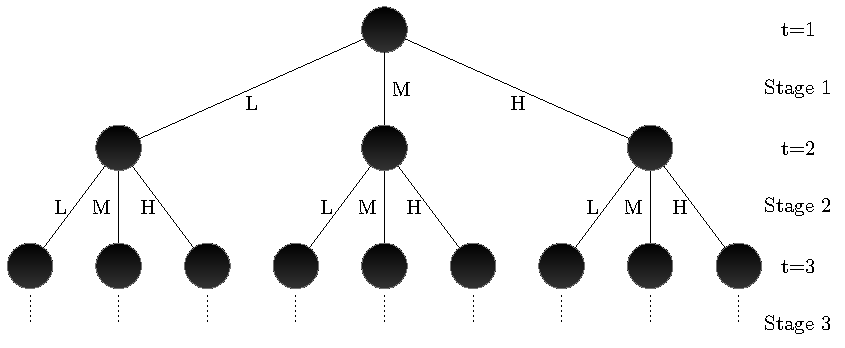
\includegraphics{Figures/figure.pdf}
\caption{Scenario tree based on \cite{Wei_1}. L = low demand, M = medium demand, H = high demand }
\centering
\label{fig:scenarios}
\end{figure}
At the beginning of the first period the manager makes a decision based on the information he gets. He sees the consequences in the next period and gains new information from that. Based on this information and the demand distribution he makes decisions in the second period for the third period. The same process is then used for the other periods as well. For each scenario tree the optimal solution can be determined. The number of scenarios is given by $\Omega^{T-1}$.
